\documentclass{article}\usepackage[]{graphicx}\usepackage[]{color}
%% maxwidth is the original width if it is less than linewidth
%% otherwise use linewidth (to make sure the graphics do not exceed the margin)
\makeatletter
\def\maxwidth{ %
  \ifdim\Gin@nat@width>\linewidth
    \linewidth
  \else
    \Gin@nat@width
  \fi
}
\makeatother

\definecolor{fgcolor}{rgb}{0.345, 0.345, 0.345}
\newcommand{\hlnum}[1]{\textcolor[rgb]{0.686,0.059,0.569}{#1}}%
\newcommand{\hlstr}[1]{\textcolor[rgb]{0.192,0.494,0.8}{#1}}%
\newcommand{\hlcom}[1]{\textcolor[rgb]{0.678,0.584,0.686}{\textit{#1}}}%
\newcommand{\hlopt}[1]{\textcolor[rgb]{0,0,0}{#1}}%
\newcommand{\hlstd}[1]{\textcolor[rgb]{0.345,0.345,0.345}{#1}}%
\newcommand{\hlkwa}[1]{\textcolor[rgb]{0.161,0.373,0.58}{\textbf{#1}}}%
\newcommand{\hlkwb}[1]{\textcolor[rgb]{0.69,0.353,0.396}{#1}}%
\newcommand{\hlkwc}[1]{\textcolor[rgb]{0.333,0.667,0.333}{#1}}%
\newcommand{\hlkwd}[1]{\textcolor[rgb]{0.737,0.353,0.396}{\textbf{#1}}}%
\let\hlipl\hlkwb

\usepackage{framed}
\makeatletter
\newenvironment{kframe}{%
 \def\at@end@of@kframe{}%
 \ifinner\ifhmode%
  \def\at@end@of@kframe{\end{minipage}}%
  \begin{minipage}{\columnwidth}%
 \fi\fi%
 \def\FrameCommand##1{\hskip\@totalleftmargin \hskip-\fboxsep
 \colorbox{shadecolor}{##1}\hskip-\fboxsep
     % There is no \\@totalrightmargin, so:
     \hskip-\linewidth \hskip-\@totalleftmargin \hskip\columnwidth}%
 \MakeFramed {\advance\hsize-\width
   \@totalleftmargin\z@ \linewidth\hsize
   \@setminipage}}%
 {\par\unskip\endMakeFramed%
 \at@end@of@kframe}
\makeatother

\definecolor{shadecolor}{rgb}{.97, .97, .97}
\definecolor{messagecolor}{rgb}{0, 0, 0}
\definecolor{warningcolor}{rgb}{1, 0, 1}
\definecolor{errorcolor}{rgb}{1, 0, 0}
\newenvironment{knitrout}{}{} % an empty environment to be redefined in TeX

\usepackage{alltt}
\input{c:/aaaWork/zGnrlLatex/GnrlPreamble}
\input{c:/aaaWork/zGnrlLatex/justRPreamble}
\hypersetup{pdftitle = Final Exam Key -- LakeSurvey}
\IfFileExists{upquote.sty}{\usepackage{upquote}}{}
\begin{document}
\section*{Final Exam Key -- LakeSurvey}


\begin{knitrout}
\definecolor{shadecolor}{rgb}{0.969, 0.969, 0.969}\color{fgcolor}\begin{kframe}
\begin{verbatim}
       n   nvalid     mean       sd      min       Q1   median       Q3      max 
  1553.0   1511.0     36.9     32.8      0.0      8.0     28.0     50.0    200.0 
percZero 
     0.6 
\end{verbatim}
\end{kframe}

{\centering 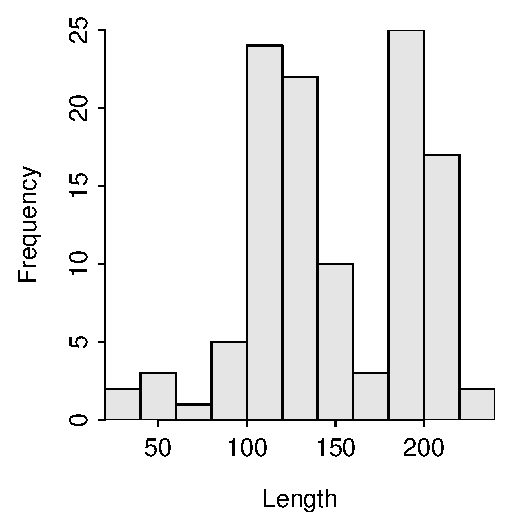
\includegraphics[width=.4\linewidth]{Figs/unnamed-chunk-1-1} 

}



\end{knitrout}
\begin{knitrout}
\definecolor{shadecolor}{rgb}{0.969, 0.969, 0.969}\color{fgcolor}\begin{kframe}
\begin{verbatim}

    ltHS       HS someColl  College GradProf 
     1.0     13.2     20.3     32.6     32.9 
\end{verbatim}
\end{kframe}
\end{knitrout}
\begin{knitrout}
\definecolor{shadecolor}{rgb}{0.969, 0.969, 0.969}\color{fgcolor}\begin{kframe}
\begin{verbatim}
The correlation is 0.205
\end{verbatim}
\end{kframe}

{\centering 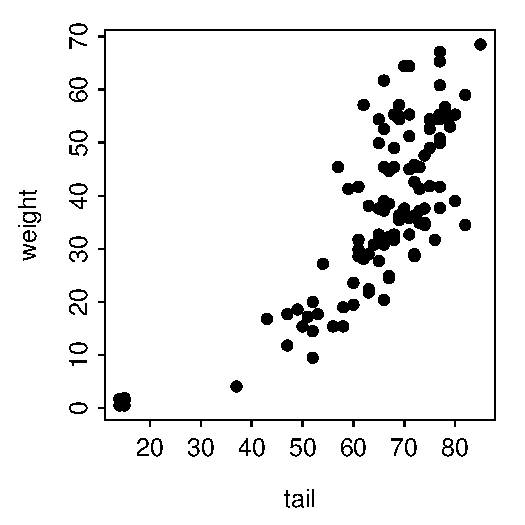
\includegraphics[width=.4\linewidth]{Figs/unnamed-chunk-3-1} 

}



\end{knitrout}
\begin{knitrout}
\definecolor{shadecolor}{rgb}{0.969, 0.969, 0.969}\color{fgcolor}\begin{kframe}
\begin{verbatim}
(Intercept)         age 
  2.7375078   0.5720521 
The predicted value at a median of 60 is 37.061
The residual is 35 - 48.502 = -13.502
The r-squared value is 0.042
\end{verbatim}
\end{kframe}
\end{knitrout}

\clearpage
\begin{knitrout}
\definecolor{shadecolor}{rgb}{0.969, 0.969, 0.969}\color{fgcolor}\begin{kframe}
\begin{verbatim}
     
      0_days 1_6_days 7_14_days 15_30_days 30_60_days 60+_days
  No      81      180       247        334        180       68
  Yes     38       78        59         74         53       77
     
        0_days  1_6_days 7_14_days 15_30_days 30_60_days 60+_days
  No  88.29816 191.43635 227.05242   302.7366  172.88632 107.5902
  Yes 30.70184  66.56365  78.94758   105.2634   60.11368  37.4098
\end{verbatim}
\end{kframe}
\end{knitrout}
\begin{knitrout}
\definecolor{shadecolor}{rgb}{0.969, 0.969, 0.969}\color{fgcolor}\begin{kframe}
\begin{verbatim}
Pearson's Chi-squared test with table(df$prmryRes, df$fishing) 
X-squared = 81.8929, df = 5, p-value = 3.37e-16
\end{verbatim}
\end{kframe}
\end{knitrout}
\begin{knitrout}
\definecolor{shadecolor}{rgb}{0.969, 0.969, 0.969}\color{fgcolor}\begin{kframe}
\begin{verbatim}
Levene's Test for Homogeneity of Variance (center = median)
        Df F value Pr(>F)
group    1  0.3034 0.5818
      1335               
\end{verbatim}
\end{kframe}
\end{knitrout}
\begin{knitrout}
\definecolor{shadecolor}{rgb}{0.969, 0.969, 0.969}\color{fgcolor}\begin{kframe}
\begin{verbatim}
 Two Sample t-test with value by prmryRes 
t = -2.1221, df = 1335, p-value = 0.03401
alternative hypothesis: true difference in means is not equal to 0 
95 percent confidence interval:
 -102630.98   -4029.76 
sample estimates:
 mean in group No mean in group Yes 
         377935.9          431266.3 
\end{verbatim}
\end{kframe}
\end{knitrout}

\end{document}
